\section{Visualisierungen}

\subsection{Analyse der Anwendungsaufgaben}

Analysieren sie die konkreten Anwendungsaufgaben, die die Lösung des Zielproblems durch die Anwender:innen bearbeitet werden müssen. 
Welche sinnvollen mentale Modelle helfen den Personen bei der Bearbeitung. 
%Welche Visualisierungen helfen den Personen, die die Software verwenden, sinnvolle mentale Modelle aufzubauen. 
Sind diese mentalen Modelle für sie notwendig, um die Aufgaben lösen zu können? Gehen sie bei ihrer Argumentation von den Anwendungsaufgaben aus und kommen sie dann zu den mentalen Modellen, deren Aufbau durch Visualisierungen unterstützt wird. 
\subsection{Anforderungen an die Visualisierungen}

Bei diesem Visualisierungsprojekt sind klare Anforderungen an die Darstellung von Daten von entscheidender Bedeutung. Um potenziellen Käufern eine hilfreiche Entscheidungsgrundlage zu bieten, sollten die Visualisierungen Aspekte wie Fahrzeugpreise, Kilometerstand, Baujahr, etc. einschließen. Eine intuitive Benutzeroberfläche ist unabdingbar, damit die Interessenten mühelos durch die Vielzahl von Angeboten navigieren können. Die Visualisierungen sollten daher die Möglichkeit bieten, Fahrzeuge anhand verschiedener Parameter zu filtern und zu vergleichen. Ein interaktiver Ansatz mit Filteroptionen und Hover-Funktionen könnte dabei helfen, detaillierte Informationen zu einzelnen Fahrzeugen abzurufen. Die visuelle Darstellung sollte sowohl informativ als auch ansprechend sein, um die Benutzererfahrung zu optimieren und eine effektive Entscheidungsfindung zu ermöglichen.  \\
Basierend auf diesen Metaanforderungen werden konkrete User Stories formuliert, die im Rahmen des Projektes addressiert werden sollen. \\
Funktionale User Stories: \\
\begin{enumerate}

    \item Als Nutzer möchte  Fahrzeuge anhand verschiedener Parameter wie Preis, Kilometerstand und Baujahr zu vergleichen, um schnell einen Überblick über die verfügbaren Optionen zu erhalten.
    
    \item Als Nutzer wünsche ich mir einen benutzerfreundlichen Parallelplot, der alle relevanten Informationen zu einzelnen Fahrzeugen auf einen Blick darstellt. Damit kann ich die Zusammenhänge zwischen den verschiedenen Parametern besser verstehen und gezielt nach meinen Präferenzen filtern.
    
    \item Als Nutzer interessiere ich mich für einen Star Plot, der mir eine visuelle Zusammenfassung der wichtigsten Merkmale verschiedener Fahrzeugmarken bietet. Dadurch kann ich schnell erkennen, wie sich die Marken in Bezug auf verschiedene Parameter unterscheiden.
\end{enumerate}
Nichtfunktionale User Stories: \\
\begin{enumerate}
    \item Als Anwender möchte ich eine ansprechende und intuitive Oberfläche erleben, die meine Navigation durch die Gebrauchtwagenanzeigen erleichtert. Die Visualisierungen sollten informativ und leicht verständlich sein, um mir eine effiziente Entscheidungsfindung zu ermöglichen.
    
    \item Als Nutzer erwarte ich, dass die Visualisierungen eine hohe Benutzerfreundlichkeit bieten, einschließlich interaktiver Elemente wie Filteroptionen und Hover-Funktionen. Dadurch kann ich gezielt nach meinen Anforderungen suchen und zusätzliche Details zu einzelnen Fahrzeugen abrufen.
    
    \item Als Anwender möchte ich die Möglichkeit haben, die Visualisierungen individuell anzupassen, indem ich verschiedene Parameter auswähle oder abwähle. Dadurch kann ich meine Suche und Analyse personalisieren und mich auf die für mich relevanten Informationen konzentrieren.
    
\end{enumerate}



\begin{figure}[h]
    \centering
    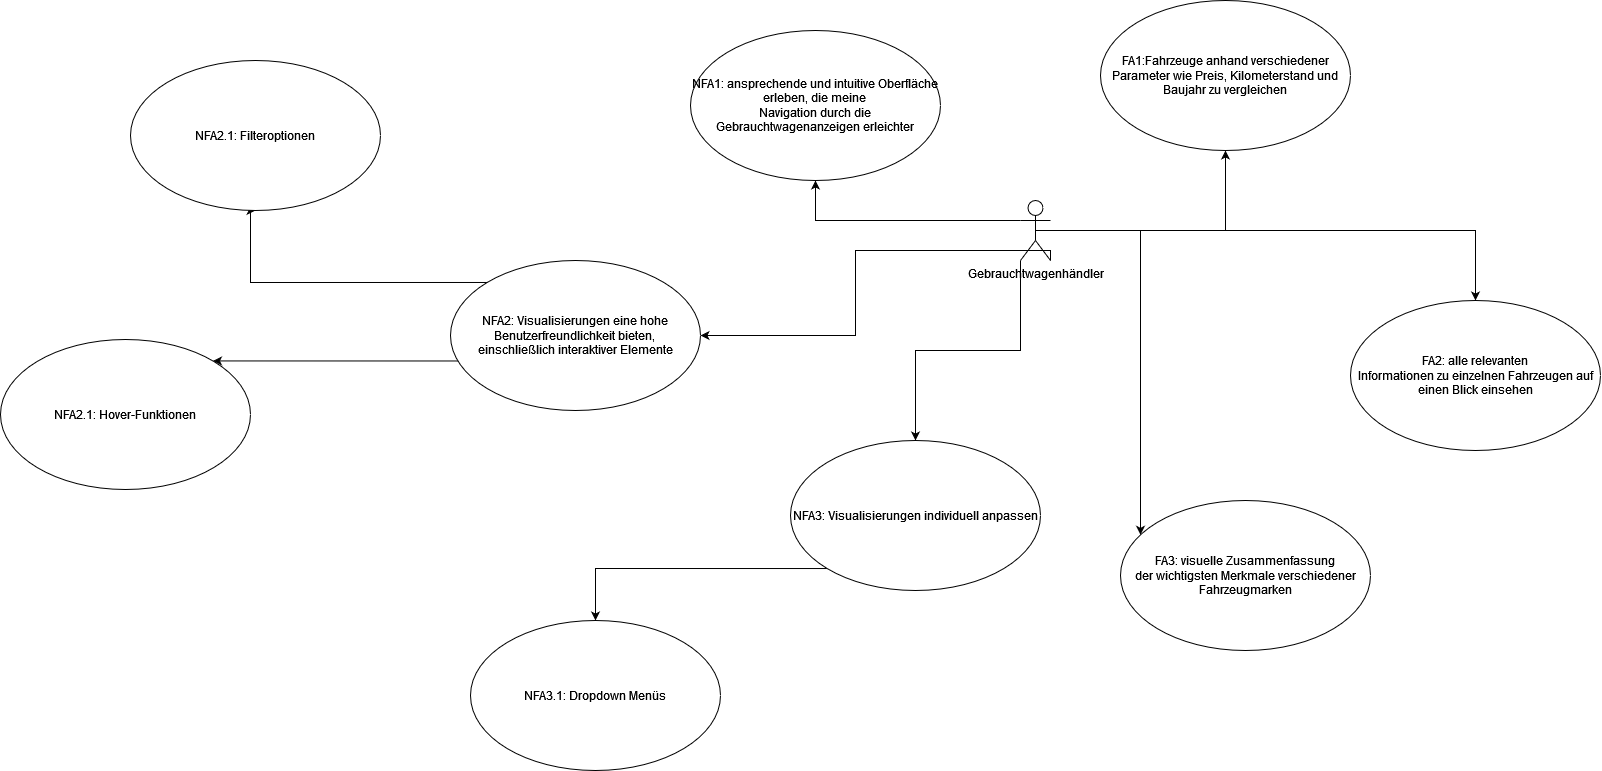
\includegraphics[width = \textwidth]{img/uc_diagram.png}
    \caption{Use Case Diagramm}
    \label{fig:uc_diagram}
\end{figure}

Aus diesen User Stories wurden dann funktionale und nicht funktionale Anforderungen in einem Use-Case Diagramm (Abbildung \ref*{fig:uc_diagram}) erstellt. \\
\subsection{Präsentation der Visualisierungen}
\subsubsection{Visualisierung Eins}

Der Scatterplot wurde entworfen, um Muster in den Gebrauchtwagenanzeigen aufzuzeigen und die Verteilung der Fahrzeuge in Bezug auf verschiedene Dimensionen sichtbar zu machen. Die Anpassung der X- und Y-Achsen kann über Dropdown-Menüs erfolgen, um eine direkte Vergleichsmöglichkeit von zwei Größen zu ermöglichen.\\

\begin{figure}[H]
    \centering
    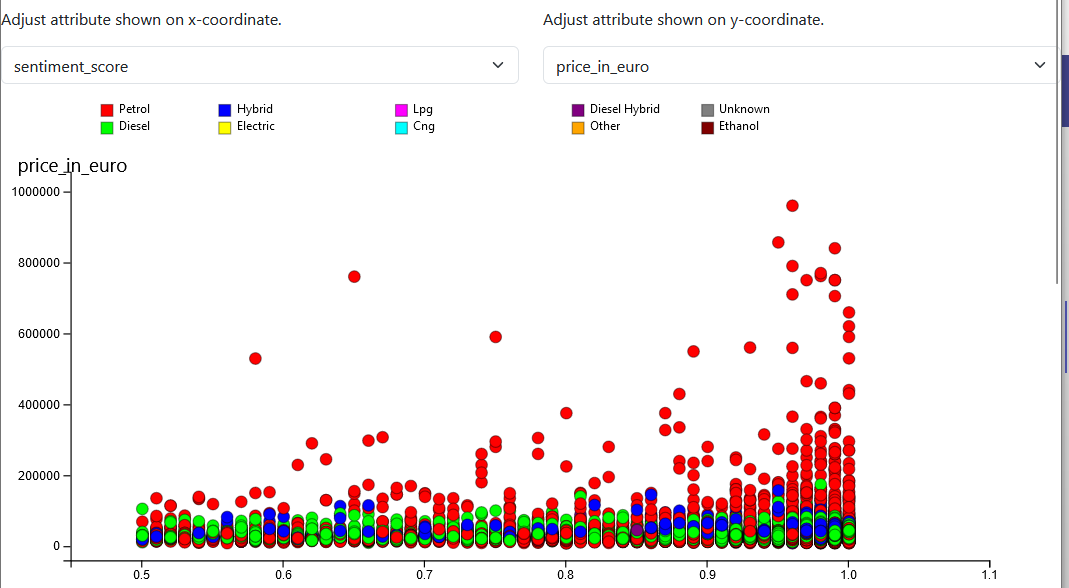
\includegraphics[width = \textwidth]{img/scatterplot.png}
    \caption{Scatterplot}
    \label{fig:scatter}
\end{figure}
\subsubsection{Visualisierung Zwei}

Im Parallelplot können mehrere Dimensionen gleichzeitig betrachtet werden, und die Linienverläufe zwischen den Achsen können auf mögliche Zusammenhänge hinweisen. \\
Die Anpassung der Achsen und Dimensionen im Parallelplot kann durch Auswahl der relevanten Attribute erfolgen. Dabei ermöglicht die visuelle Darstellung der Linienverläufe eine direkte Vergleichbarkeit verschiedener Fahrzeuge in Bezug auf diese Attribute. \\
Zusätzlich kann ein Datenpunkt mittels hovern eingefärbt werden. Dies erhöht die Bedienbarkeit. \\

\begin{figure}[H]
    \centering
    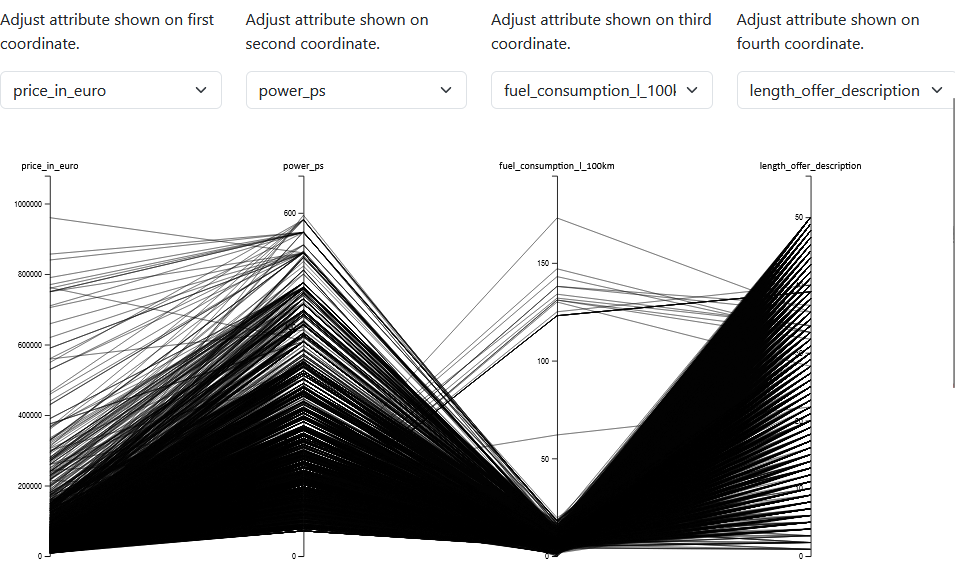
\includegraphics[width = \textwidth]{img/parallelplot.png}
    \caption{Parallelplot}
    \label{fig:scatter}
\end{figure}


\subsubsection{Visualisierung Drei}

Der Starplot bietet eine umfassende Visualisierung aller Attribute von Automobilanzeigen einer bestimmten Marke auf der Plattform. Durch diese Darstellung lassen sich alle relevanten Merkmale gleichzeitig betrachten und erleichtern somit einen schnellen Überblick. \\
Die Achsen des Starplots repräsentieren die verschiedenen Attribute, auf denen die durchschnittliche / summierte Attributsausprägung aller Anzeigen von Autos dieser Marke dargestellt ist. Dies ermöglicht einen schnellen Überblick über die Attributen dieser Marke. \\
Um den Starplot zu verwenden, wählen Sie die gewünschte Automarke aus, und der Plot wird automatisch generiert. Die Positionen der Linien auf den Achsen vermitteln Informationen über die relativen Werte der Attribute für jedes Fahrzeug. \\
Insgesamt ermöglicht der Starplot eine effektive und schnelle visuelle Analyse der Attribute aller Fahrzeuge einer ausgewählten Marke auf der Plattform. \\

\begin{figure}[H]
    \centering
    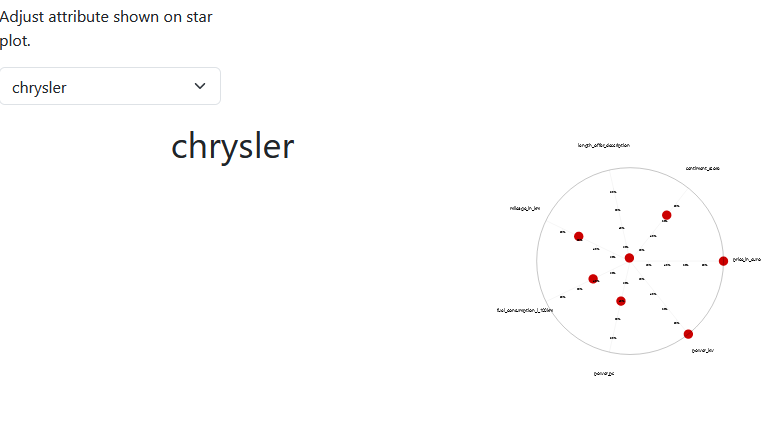
\includegraphics[width = \textwidth]{img/starplot.png}
    \caption{Starplot}
    \label{fig:scatter}
\end{figure}


\subsection{Interaktion}


Die Interaktion mit den Visualisierungen ist ein zentraler Aspekt des Projekts. Ein übergeordnetes Ziel besteht darin, alle Visualisierungen auf einer Seite anzuordnen, sodass ein einfaches Scrollen zwischen ihnen einen schnellen Gesamtüberblick ermöglicht. Um die Benutzererfahrung zu verbessern und die Visualisierungen an die Bedürfnisse des Nutzers anzupassen, sind verschiedene Anpassungsmöglichkeiten implementiert. \\

Insbesondere bieten das Scatterplot und das Parallelplot die Möglichkeit zur Anpassung durch einen Schieberegler (siehe Abbildung \ref{fig:schieber}). Durch Auswahl einer Jahreszahl werden in beiden Grafiken nur Daten aus diesem Jahr angezeigt. Diese Anpassung ist nicht nur benutzerfreundlich, sondern dient auch der Optimierung, da die Visualisierung aller Daten auf einmal zu langen Wartezeiten führen könnte. \\

Zusätzlich ermöglicht das Scatterplot eine weitere Anpassung durch zwei Drop-Down-Menüs. Diese Menüs dienen der Auswahl der Daten für die x- und y-Achse. Die Interaktion mit dem Scatterplot umfasst auch vier Dropdowns, jeweils für jede Achse. Durch diese Interaktion werden nicht alle verfügbaren Daten angezeigt, sondern nur die vom Nutzer gewünschten Werte. Dies trägt zur verbesserten Übersichtlichkeit und damit zur Nutzbarkeit für die Zielgruppe bei. \\
\begin{figure}[H]
    \centering
    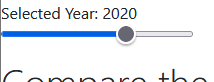
\includegraphics{img/interaktion1.png}
    \caption{Schieberegler}
    \label{fig:schieber}
\end{figure}

Die Auswahl der Daten im Parallelplot ist ähnlich möglich. Hier hat der Nutzer über vier Drop-Downs die gewünschten Daten einzubinden. \\
Auch im Starplot kann der Nutzer einen Datensatz - eine Marke - auswählen, die er/sie sich genauer anschauen will. \\